\documentclass[]{article}
\usepackage{lmodern}
\usepackage{amssymb,amsmath}
\usepackage{ifxetex,ifluatex}
\usepackage{fixltx2e} % provides \textsubscript
\ifnum 0\ifxetex 1\fi\ifluatex 1\fi=0 % if pdftex
  \usepackage[T1]{fontenc}
  \usepackage[utf8]{inputenc}
\else % if luatex or xelatex
  \ifxetex
    \usepackage{mathspec}
  \else
    \usepackage{fontspec}
  \fi
  \defaultfontfeatures{Ligatures=TeX,Scale=MatchLowercase}
\fi
% use upquote if available, for straight quotes in verbatim environments
\IfFileExists{upquote.sty}{\usepackage{upquote}}{}
% use microtype if available
\IfFileExists{microtype.sty}{%
\usepackage[]{microtype}
\UseMicrotypeSet[protrusion]{basicmath} % disable protrusion for tt fonts
}{}
\PassOptionsToPackage{hyphens}{url} % url is loaded by hyperref
\usepackage[unicode=true]{hyperref}
\hypersetup{
            pdftitle={confirm-moving-render.md},
            pdfborder={0 0 0},
            breaklinks=true}
\urlstyle{same}  % don't use monospace font for urls
\usepackage{longtable,booktabs}
% Fix footnotes in tables (requires footnote package)
\IfFileExists{footnote.sty}{\usepackage{footnote}\makesavenoteenv{long table}}{}
\usepackage{graphicx,grffile}
\makeatletter
\def\maxwidth{\ifdim\Gin@nat@width>\linewidth\linewidth\else\Gin@nat@width\fi}
\def\maxheight{\ifdim\Gin@nat@height>\textheight\textheight\else\Gin@nat@height\fi}
\makeatother
% Scale images if necessary, so that they will not overflow the page
% margins by default, and it is still possible to overwrite the defaults
% using explicit options in \includegraphics[width, height, ...]{}
\setkeys{Gin}{width=\maxwidth,height=\maxheight,keepaspectratio}
\IfFileExists{parskip.sty}{%
\usepackage{parskip}
}{% else
\setlength{\parindent}{0pt}
\setlength{\parskip}{6pt plus 2pt minus 1pt}
}
\setlength{\emergencystretch}{3em}  % prevent overfull lines
\providecommand{\tightlist}{%
  \setlength{\itemsep}{0pt}\setlength{\parskip}{0pt}}
\setcounter{secnumdepth}{0}
% Redefines (sub)paragraphs to behave more like sections
\ifx\paragraph\undefined\else
\let\oldparagraph\paragraph
\renewcommand{\paragraph}[1]{\oldparagraph{#1}\mbox{}}
\fi
\ifx\subparagraph\undefined\else
\let\oldsubparagraph\subparagraph
\renewcommand{\subparagraph}[1]{\oldsubparagraph{#1}\mbox{}}
\fi

% set default figure placement to htbp
\makeatletter
\def\fps@figure{htbp}
\makeatother


\title{confirm-moving-render.md}
\date{}

\begin{document}
\maketitle

\section{見出し}\label{header-n219}

\begin{itemize}
\item
  IN
\end{itemize}

\begin{verbatim}
# 見出し1
## 見出し2
### 見出し3
#### 見出し4
##### 見出し5
###### 見出し6
\end{verbatim}

\begin{itemize}
\item
  OUT
\end{itemize}

\section{見出し1}\label{header-n228}

\subsection{見出し2}\label{header-n229}

\subsubsection{見出し3}\label{header-n230}

\paragraph{見出し4}\label{header-n231}

\subparagraph{見出し5}\label{header-n232}

見出し6

\section{色コード}\label{header-n235}

\begin{itemize}
\item
  IN
\end{itemize}

\begin{verbatim}
![](https://via.placeholder.com/16/c7e7f6/FFFFFF/?text=%20) `#c7e7f6`
![](https://via.placeholder.com/16/abdbf1/FFFFFF/?text=%20) `#abdbf1`
![](https://via.placeholder.com/16/6ec1e9/FFFFFF/?text=%20) `#6ec1e9`
![](https://via.placeholder.com/16/47b1e1/FFFFFF/?text=%20) `#47b1e1`
![](https://via.placeholder.com/16/0093d6/FFFFFF/?text=%20) `#0093d6`
![](https://via.placeholder.com/16/221816/FFFFFF/?text=%20) `#221816`
\end{verbatim}

\begin{itemize}
\item
  OUT
\end{itemize}

\includegraphics{https://via.placeholder.com/16/c7e7f6/FFFFFF/?text= }
\texttt{\#c7e7f6}\\
\includegraphics{https://via.placeholder.com/16/abdbf1/FFFFFF/?text= }
\texttt{\#abdbf1}\\
\includegraphics{https://via.placeholder.com/16/6ec1e9/FFFFFF/?text= }
\texttt{\#6ec1e9}\\
\includegraphics{https://via.placeholder.com/16/47b1e1/FFFFFF/?text= }
\texttt{\#47b1e1}\\
\includegraphics{https://via.placeholder.com/16/0093d6/FFFFFF/?text= }
\texttt{\#0093d6}\\
\includegraphics{https://via.placeholder.com/16/221816/FFFFFF/?text= }
\texttt{\#221816}

\section{インラインコード}\label{header-n244}

\begin{itemize}
\item
  IN
\end{itemize}

\begin{verbatim}
これは `echo うんこ`です。
\end{verbatim}

\begin{itemize}
\item
  OUT
\end{itemize}

これは \texttt{echo\ うんこ}です。

\section{ノンインラインコード}\label{header-n254}

\begin{itemize}
\item
  IN
\end{itemize}

\begin{verbatim}

```

#!/usr/bin/env bash


echo うんこ

```
\end{verbatim}

\begin{itemize}
\item
  OUT
\end{itemize}

\begin{verbatim}

#!/usr/bin/env bash


echo うんこ
\end{verbatim}

\section{ノンオーダリスト}\label{header-n266}

\begin{itemize}
\item
  IN
\end{itemize}

\begin{verbatim}
- リスト1
    - リスト1-1
        - リスト1-1-1
        - リスト1-1-2
    - リスト1-2
- リスト2
- リスト3
\end{verbatim}

\begin{itemize}
\item
  OUT
\item
  リスト1

  \begin{itemize}
  \item
    リスト1-1

    \begin{itemize}
    \item
      リスト1-1-1
    \item
      リスト1-1-2
    \end{itemize}
  \item
    リスト1-2
  \end{itemize}
\item
  リスト2
\item
  リスト3
\end{itemize}

\section{オーダリスト}\label{header-n290}

\begin{itemize}
\item
  IN
\end{itemize}

\begin{verbatim}
1. 番号付きリスト1
    1. 番号付きリスト1-1
    1. 番号付きリスト1-2
1. 番号付きリスト2
1. 番号付きリスト3
\end{verbatim}

\begin{itemize}
\item
  OUT
\end{itemize}

\begin{enumerate}
\def\labelenumi{\arabic{enumi}.}
\item
  番号付きリスト1

  \begin{enumerate}
  \def\labelenumii{\arabic{enumii}.}
  \item
    番号付きリスト1-1
  \item
    番号付きリスト1-2
  \end{enumerate}
\item
  番号付きリスト2
\item
  番号付きリスト3
\end{enumerate}

\section{引用}\label{header-n310}

\begin{itemize}
\item
  IN
\end{itemize}

\begin{verbatim}

> **Note:**  Interfere when the enemy is making a mistake.
\end{verbatim}

\begin{itemize}
\item
  OUT
\end{itemize}

\begin{quote}
\textbf{Note:} Interfere when the enemy is making a mistake.
\end{quote}

\section{リンク}\label{header-n322}

\begin{itemize}
\item
  IN
\end{itemize}

\begin{verbatim}
[pngフリー画像集](https://www.pngonly.com/owl-png/)
\end{verbatim}

\begin{itemize}
\item
  OUT
\end{itemize}

\href{https://www.pngonly.com/owl-png/}{pngフリー画像集}

\section{強調表示}\label{header-n331}

\begin{itemize}
\item
  IN
\end{itemize}

\begin{verbatim}
これは **うんこ** です
\end{verbatim}

\begin{itemize}
\item
  OUT
\end{itemize}

これは \textbf{うんこ} です

\section{画像}\label{header-n341}

\begin{verbatim}
curl -sSLO https://www.pngonly.com/wp-content/uploads/2017/06/Owl-Close-PNG-Photo.png
\end{verbatim}

\begin{itemize}
\item
  IN
\end{itemize}

\begin{verbatim}

![フクロウ](./Owl-Close-PNG-Photo.png "Owl")
\end{verbatim}

\begin{itemize}
\item
  OUT
\end{itemize}

\begin{figure}
\centering
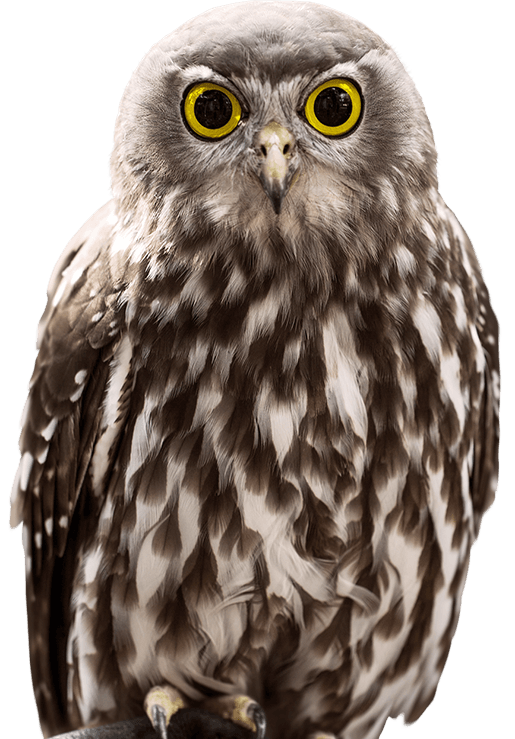
\includegraphics{/home/kuraine/script-sketch/Typora/Owl-Close-PNG-Photo.png}
\caption{Owl}
\end{figure}

\section{テーブル}\label{header-n353}

\begin{itemize}
\item
  IN
\end{itemize}

\begin{verbatim}
|                  | ASCII                           | HTML                          |
| ---------------- | ------------------------------- | ----------------------------- |
| Single backticks | `'Isn't this fun?'`             | 'Isn't this fun?'             |
| Quotes           | `"Isn't this fun?"`             | "Isn't this fun?"             |
| Dashes           | `-- is en-dash, --- is em-dash` | -- is en-dash, --- is em-dash |
\end{verbatim}

\begin{itemize}
\item
  OUT
\end{itemize}

\begin{longtable}[]{@{}lll@{}}
\toprule
& ASCII & HTML\tabularnewline
\midrule
\endhead
Single backticks &
\texttt{\textquotesingle{}Isn\textquotesingle{}t\ this\ fun?\textquotesingle{}}
& 'Isn't this fun?'\tabularnewline
Quotes & \texttt{"Isn\textquotesingle{}t\ this\ fun?"} & "Isn't this
fun?"\tabularnewline
Dashes & \texttt{-\/-\ is\ en-dash,\ -\/-\/-\ is\ em-dash} & -\/- is
en-dash, -\/-\/- is em-dash\tabularnewline
\bottomrule
\end{longtable}

\begin{itemize}
\item
  IN
\end{itemize}

\begin{verbatim}
| 左揃え | 中央揃え | 右揃え |
|:--|:--:|--:|
|1 |2 |3 |
|4 |5 |6 |
\end{verbatim}

\begin{itemize}
\item
  OUT
\end{itemize}

\begin{longtable}[]{@{}lll@{}}
\toprule
左揃え & 中央揃え & 右揃え\tabularnewline
\midrule
\endhead
1 & 2 & 3\tabularnewline
4 & 5 & 6\tabularnewline
\bottomrule
\end{longtable}

\begin{itemize}
\item
  IN
\end{itemize}

\begin{verbatim}

|`code`    |*italic*                  |
|:--:|:--:|
|**bold**  |***bold italic***         |
|$ omega $|[Qiita](http://qiita.com)|
\end{verbatim}

\begin{itemize}
\item
  OUT
\end{itemize}

texうまくいかんな

\begin{longtable}[]{@{}ll@{}}
\toprule
\texttt{code} & \emph{italic}\tabularnewline
\midrule
\endhead
\textbf{bold} & \textbf{\emph{bold italic}}\tabularnewline
\$ omega \$ & \href{http://qiita.com}{Qiita}\tabularnewline
\bottomrule
\end{longtable}

\section{tex}\label{header-n423}

\begin{itemize}
\item
  https://qiita.com/MuAuan/items/64dc82030a9ec4f5cef9
\end{itemize}

The \emph{Gamma function} satisfying \$\textbackslash{}Gamma(n) =
(n-1)!\textbackslash{}quad\textbackslash{}forall
n\textbackslash{}in\textbackslash{}mathbb N\$ is via the Euler integral

\[\Gamma(z) = \int_0^\infty t^{z-1}e^{-t}dt\,.\]

\begin{quote}
You can find more information about \textbf{LaTeX} mathematical
expressions
\href{http://meta.math.stackexchange.com/questions/5020/mathjax-basic-tutorial-and-quick-reference}{here}.
\end{quote}

\section{UML diagrams}\label{header-n432}

これはvscodeでdraw.ioができるようになったから、あんま使わんかも??

You can render UML diagrams using
\href{https://mermaidjs.github.io/}{Mermaid}. For example, this will
produce a sequence diagram:

\begin{figure}
\centering
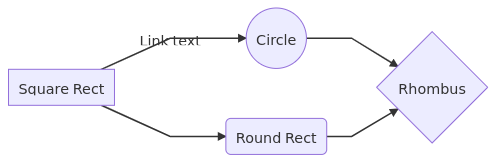
\includegraphics[width=6.93750in]{1590755747410.png}
\caption{}\label{mermaid}
\end{figure}

And this will produce a flow chart:

\begin{figure}
\centering
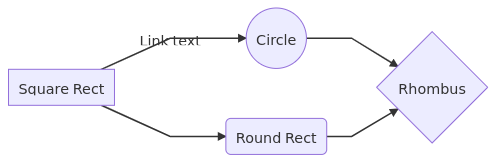
\includegraphics[width=5.16667in]{1590755747410.png}
\caption{}\label{mermaid}
\end{figure}

\end{document}
